% ======================================================================
%  Chapter 1 — The Problem of Robust Light
% ======================================================================

\section{Light that cannot turn back}
\label{sec:ch1-cannot-turn-back}

Every optical engineer knows that light reflects.  A fibre splice, a
waveguide bend, a scratch on a mirror---any interruption of the medium
sends part of the wave backward.  In most of photonics this is merely a
nuisance, compensated by isolators, circulators, or careful impedance
matching.  But suppose we could build a channel for electromagnetic
energy in which backward propagation is \emph{structurally forbidden}:
not suppressed by a clever design trick that might fail under
perturbation, but eliminated by a mathematical property of the
electromagnetic band structure itself.  What would the Maxwell equations
have to contain for such a channel to exist?

That question is the starting point of this book.  The answer, as we
shall develop in detail over the coming chapters, involves a remarkable
convergence of ideas from nineteenth-century electromagnetism,
twentieth-century condensed-matter physics, and twenty-first-century
photonic-crystal engineering.  The key concept is \emph{topology}:
certain integer-valued invariants of the photonic band structure that
cannot change under smooth deformations of the medium, and that
guarantee the existence of unidirectional interface modes whenever two
media with different invariants are brought together.

Before we can state this precisely, however, we need to see why ordinary
approaches to waveguide robustness fail, and what new ingredient the
problem demands.

\section{Backscattering in ordinary waveguides}
\label{sec:ch1-backscattering}

Consider a conventional dielectric slab waveguide: a high-index core of
thickness $d$ and refractive index $n_1$ sandwiched between cladding
layers of index $n_2 < n_1$.  Guided modes exist when the transverse
resonance condition is satisfied, and for a given frequency $\omega$
there are generally both forward-propagating modes (with propagation
constant $+\beta$) and backward-propagating modes (with $-\beta$).
The dispersion relation $\omega(\beta)$ is symmetric:
$\omega(\beta)=\omega(-\beta)$.

This symmetry is a direct consequence of \emph{time-reversal
invariance}.  Maxwell's equations in a lossless, non-magnetic dielectric
are invariant under the operation $t\to -t$, which sends
$\Efield\to\Efield$, $\Hfield\to-\Hfield$, and
$\beta\to-\beta$.  If a forward mode at $(\omega,+\beta)$ exists, then
time reversal produces a backward mode at $(\omega,-\beta)$.

The physical consequence is immediate: any perturbation that couples the
forward and backward channels---a surface roughness, a point defect, a
bend whose radius of curvature is comparable to the wavelength---can
scatter light from $+\beta$ to $-\beta$.  No matter how carefully
the waveguide is fabricated, backscattering is always \emph{allowed} by
symmetry.  We can reduce it; we cannot forbid it.

\subsection{A quantitative reminder}
\label{sec:ch1-backscattering-quantitative}

To make this concrete, recall the coupled-mode estimate for
backscattering loss in a single-mode waveguide with sidewall roughness.
If the roughness has root-mean-square amplitude $\sigma$ and correlation
length $L_c$, the power attenuation coefficient due to backscattering
scales as
\begin{equation}\label{eq:ch1-roughness-loss}
  \alpha_{\mathrm{back}} \;\propto\;
  \frac{\sigma^2}{\lambda^2}\,
  \frac{(\Delta n)^2}{n_{\mathrm{eff}}}\,
  \frac{L_c}{1 + (2\beta L_c)^2}\,,
\end{equation}
where $\Delta n = n_1-n_2$ is the index contrast and
$n_{\mathrm{eff}}=\beta c/\omega$ is the effective index.
The essential point is that $\alpha_{\mathrm{back}}>0$ for any nonzero
$\sigma$: the backward channel is always open.

In silicon photonic waveguides at telecom wavelengths, typical
propagation losses from scattering are of order
$1$--$3\;\mathrm{dB\,cm}^{-1}$ even in state-of-the-art fabrication.
This is tolerable for short on-chip interconnects, but it sets a
fundamental limit on the quality factor of ring resonators, the
coherence length of delay lines, and the dynamic range of interferometric
sensors.

\section{What would it take?}
\label{sec:ch1-what-would-it-take}

The existence of a backward channel is guaranteed by time-reversal
symmetry.  To eliminate it, we must either break time-reversal symmetry
or find a more subtle structural mechanism that effectively decouples
the two propagation directions.

\paragraph{Breaking time reversal.}
In electromagnetism, time-reversal symmetry is broken by
magneto-optical (Faraday) media: materials whose permittivity or
permeability tensor acquires antisymmetric off-diagonal components
when an external magnetic bias is applied.  A familiar device
exploiting this effect is the Faraday isolator, which rotates the
polarisation of a transmitted beam by $45^{\circ}$ in a fixed
sense regardless of propagation direction.  Faraday isolators
are standard components in laser systems, but they are bulky
discrete elements, not integrated waveguiding structures.

The question, then, is whether one can embed the Faraday effect
into the \emph{band structure} of a periodic photonic medium---a
photonic crystal---in such a way that one-way propagation becomes a
property of the entire frequency band rather than a discrete device.

\paragraph{The electronic precedent.}
This question has a remarkable precedent in condensed-matter physics.
In 1980, Klaus von Klitzing discovered that the Hall conductance of a
two-dimensional electron gas in a strong magnetic field is quantised
to integer multiples of $e^2/h$, with extraordinary precision
\cite{klitzing2015method}.  Two years later, Thouless, Kohmoto, Nightingale,
and den Nijs showed that the quantisation is a consequence of a
topological invariant---the first Chern number---of the electronic
Bloch bands \cite{thouless1982quantized}.
The chiral edge states responsible for the quantised Hall current
propagate in only one direction along the sample boundary, and they
are immune to backscattering from impurities precisely because there
is no backward-propagating channel for them to scatter into.

The existence of these one-way edge states is not an accident of the
particular Hamiltonian; it is a topological consequence of the
nonzero Chern number of the filled bands.  As long as the bulk band
gap remains open, the edge states persist regardless of the details
of the boundary or the disorder.

\paragraph{From electrons to photons.}
In a landmark 2005 paper (published in 2008), Haldane and Raghu
recognised that the one-particle band-structure topology underlying the
integer quantum Hall effect has nothing essentially quantum-mechanical
about it \cite{haldane2008possible}.  It is a property of waves in
periodic media with broken time-reversal symmetry.  Since the
Maxwell normal-mode problem in a lossless periodic medium is a
generalised Hermitian eigenvalue problem---structurally analogous to the
electronic Schr\"odinger equation, though with a different inner
product---the same topological classification applies.

Haldane and Raghu considered a two-dimensional photonic crystal made of
dielectric rods with a magneto-optical (gyrotropic) response.  They
showed that:
\begin{enumerate}[label=(\roman*)]
  \item The photonic band structure of a hexagonal lattice of such rods
        generically exhibits Dirac-point degeneracies, analogous to
        those in graphene.
  \item When the gyrotropic effect lifts these degeneracies, the
        resulting bands acquire nonzero Chern numbers.
  \item At a domain wall where the sign of the gyrotropic parameter
        reverses, a unidirectional mode is bound to the interface,
        crossing the bulk band gap with a group velocity whose sign is
        fixed by the Chern-number difference across the wall.
\end{enumerate}
This is the photonic analog of the quantum Hall edge state: a one-way
waveguide, immune to backscattering, whose existence is guaranteed by
the topology of the bulk bands.

\section{The first experimental observation}
\label{sec:ch1-wang-experiment}

The theoretical prediction of Haldane and Raghu was brought to
experimental reality by Wang, Chong, Joannopoulos, and
Solja\v{c}i\'{c}, first in simulation and proposal (2008) and then in a
direct measurement (2009) \cite{nature2026observation}.
They constructed a two-dimensional photonic crystal of yttrium iron
garnet (YIG) rods in a square lattice, operating in the microwave regime
around $4.5\;\mathrm{GHz}$, and applied a static magnetic field of
approximately $0.2\;\mathrm{T}$ to magnetise the ferrite.

The key experimental observations were:
\begin{itemize}
  \item Electromagnetic energy launched into an edge channel propagated
        in only one direction around the boundary of the crystal.
  \item When a large metallic obstacle was placed in the path of the
        edge mode, the wave simply routed around the obstacle without
        any measurable reflection.  The forward transmission through
        eight lattice periods was more than five orders of magnitude
        larger than the backward signal.
  \item The one-way propagation persisted over the entire frequency
        range of the bulk band gap, not just at isolated frequencies.
\end{itemize}
These results demonstrated that the topological protection predicted
from band theory is a real, measurable electromagnetic phenomenon, not
merely a mathematical curiosity.

The geometry of the Wang experiment is shown schematically in
Figure~\ref{fig:ch1-wang}.  A square array of YIG rods sits inside a
metallic parallel-plate waveguide; an external static magnetic field
$B_0\approx 0.20$~T magnetises the ferrite and opens a topological
gap near $4.5$~GHz.  Electromagnetic energy launched along one edge of
the crystal propagates in a single direction, routing around large
metallic obstacles without any measurable backscattering.

\begin{figure}[t]
  \centering
  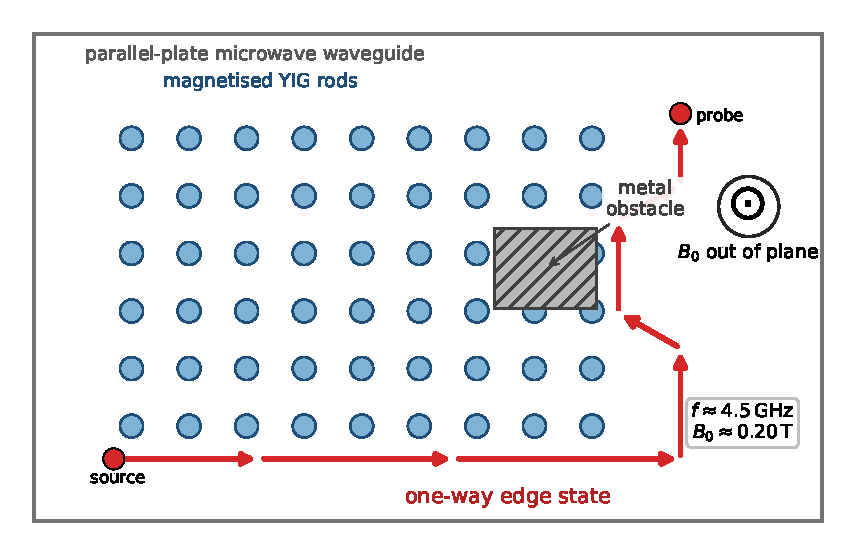
\includegraphics[width=0.88\textwidth]{figures/fig_wang_experiment_schematic.pdf}
  \caption{Schematic of the Wang et~al.\ experiment
  \cite{nature2026observation}.  A square lattice of magnetised YIG
  rods operates near $4.5$~GHz under an external bias field
  $B_0\approx 0.20$~T that breaks time-reversal symmetry.  The
  resulting gyrotropic mass, and hence the edge-state chirality, is set
  by the direction of $B_0$; the red path traces the one-way edge state routing around
  a large metallic obstacle without backscattering.}
  \label{fig:ch1-wang}
\end{figure}

\section{Why topology, and why from Maxwell?}
\label{sec:ch1-why-topology}

The preceding story can be told---and often is told---entirely in the
language of condensed-matter physics: Bloch Hamiltonians, Berry phases,
Chern numbers, bulk-boundary correspondence.  There is nothing wrong
with this; the mathematical structures are the same.  But for a book
addressed to the photonics community, and for the deepest understanding
of the physical mechanisms, we believe it is essential to derive every
topological statement directly from Maxwell's equations.

There are several reasons for this insistence.

\paragraph{The inner product is different.}
In quantum mechanics, the Hilbert-space inner product is the standard
$L^2$ integral: $\langle\psi|\phi\rangle=\int\psi^*\phi\,\dd^3 r$.
In electromagnetism, the physically correct inner product involves the
material response.  For a lossless nondispersive medium characterised by
the $6\times 6$ material matrix $\Mmat$, the electromagnetic energy
inner product is
\begin{equation}\label{eq:ch1-em-inner-product}
  \emip{\emfield_1}{\emfield_2}
  = \int \emfield_1^\dagger(\rvec)\cdot \Mmat(\rvec)\cdot
         \emfield_2(\rvec)\,\dd^3 r\,,
\end{equation}
where $\emfield = (\Efield,\Hfield)^T$ is the six-component
electromagnetic field.  Every formula for Berry connection, Berry
curvature, and Chern number must be written with respect to this inner
product, not the standard one.  Getting this wrong leads to
non-gauge-invariant expressions and incorrect topological invariants.

When the medium is dispersive---as all real magneto-optical media
are---the inner product must be further modified to incorporate the
electromagnetic energy stored in the material polarisation, leading to
the \emph{energy metric}
$\Mgmat(\omega)=\partial_\omega[\omega\Mmat(\omega)]$.  This
subtlety has no analog in the electronic problem and is easily missed
when photonic topology is derived by analogy rather than from first
principles.

\paragraph{The eigenvalue problem is generalised.}
The Maxwell normal-mode equation is not a standard eigenvalue problem
$\hat{H}\psi=E\psi$; it is a generalised eigenproblem
$\Maxop\emfield=\omega\Mmat\emfield$, with the frequency playing the
role of the eigenvalue and the material matrix appearing on the
right-hand side.  The Hermiticity (self-adjointness) that guarantees
real frequencies and orthogonal modes follows from the structure of the
Maxwell curl operator and the positivity of $\Mmat$, but the proof is
different from the quantum-mechanical case and deserves to be presented
in full.

\paragraph{Photon time reversal is bosonic.}
For electrons, the time-reversal operator satisfies $\Top^2=-1$, which
implies Kramers degeneracy and provides the symmetry protection for the
quantum spin Hall effect
\cite{kane2005sub}.  For photons, $\Top^2=+1$.  This seemingly
small algebraic difference has profound consequences: there is no
photonic Kramers theorem, and time-reversal-invariant photonic
``topological insulators'' require additional crystalline or internal
symmetries for their protection
\cite{hsieh2008topological}.  A Maxwell-first development makes this
distinction transparent from the outset.

\paragraph{Material constraints matter.}
Which materials can support topological bands?  What symmetries must be
broken, and how strong must the magneto-optical or bianisotropic
response be?  These questions can only be answered by examining the
constitutive relations directly.  A Maxwell-first approach keeps the
material physics visible at every stage, rather than hiding it behind
an effective Hamiltonian.

\section{The plan of this book}
\label{sec:ch1-plan}

This monograph develops the theory of topological photonics from the
ground up, starting from Maxwell's equations and optical energy
considerations, and building toward the full classification of
topological phases accessible to electromagnetic waves in periodic
media \cite{chen2021highlighting}.

\paragraph{Part I: Maxwell modes and optical bands.}
We begin by recasting the macroscopic Maxwell equations as a first-order
dynamical system (\chref{ch:maxwell-dynamics}), identifying the
six-component electromagnetic field and the material matrix as the
fundamental objects.  We then derive the normal-mode problem and the
electromagnetic inner product that makes it self-adjoint
(\chref{ch:normal-modes}), introduce Bloch's theorem and photonic
band structure (\chref{ch:periodic-media}), and develop the Berry
connection, Berry curvature, and Chern number for Maxwell bands
(\chref{ch:geometry-bands}).  Every formula in this part is derived from
Maxwell's equations using the correct electromagnetic inner product.

\paragraph{Part II: Chern bands and one-way waveguides.}
With the mathematical framework in place, we study the physical
mechanisms that create topological bands.  We analyse Dirac-point
degeneracies (\chref{ch:dirac-cones}), show how gyrotropic media open
topological gaps (\chref{ch:breaking-tr}), derive the one-way interface
mode at a domain wall in detail (\chref{ch:one-way-interface}), and
discuss the microwave photonic-crystal experiment that first confirmed
the prediction (\chref{ch:microwave-crystal}).  We then address the
practical problem of computing Chern numbers from numerical Maxwell
eigensolvers (\chref{ch:computing-chern}).

\paragraph{Part III: Other two-dimensional phases.}
Not all photonic topological phases require broken time-reversal
symmetry.  We discuss reciprocal designs based on pseudospin and
bianisotropy (\chref{ch:reciprocal-designs}), valley-Hall photonic
crystals (\chref{ch:valleys}), Floquet topological systems created by
temporal modulation (\chref{ch:floquet}), and one-dimensional
topological models including the photonic Su--Schrieffer--Heeger chain
(\chref{ch:one-dimension})
\cite{yang2020photonic}.

\paragraph{Part IV: Three dimensions and beyond.}
We extend the framework to three-dimensional photonic crystals with Weyl
points (\chref{ch:weyl-points}) and to synthetic dimensions created by
coupling internal degrees of freedom of resonators
(\chref{ch:synthetic-dimensions}) \cite{mancini2015observation}.

\paragraph{Part V: Imperfect, active, and nonlinear light.}
Real photonic systems have loss, gain, and nonlinearity \cite{szameit2020nonlinearity}.  We discuss
non-Hermitian topology (\chref{ch:non-hermitian}) and the emerging
frontier of nonlinear and quantum topological photonics
(\chref{ch:nonlinear-quantum})
\cite{kawabata2019symmetry}.

\paragraph{Appendices} provide supporting material on vector identities,
differential forms, numerical methods, and material-tensor conventions.

\bigskip
Throughout the book, we follow a consistent strategy: derive the key
result from Maxwell's equations first, then connect it to the
condensed-matter analogy for readers with a solid-state background, and
finally illustrate it with a concrete photonic example or experiment.
The goal is a self-contained reference that a graduate student in
photonics can read from the beginning, and that a researcher in
topological condensed matter can consult for the electromagnetic
specifics.

\section{Photonic versus electronic topology}
\label{sec:ch1-photonic-vs-electronic}

The topological ideas applied in this book were born in the study of
electron systems, but the photonic setting differs from the electronic
one in several fundamental ways.  Understanding these differences is
essential for appreciating both the power and the limitations of
topological photonics.

\subsection{Bosonic statistics and the absence of a Fermi level}
\label{sec:ch1-bosonic}

Electrons are fermions: the Pauli exclusion principle guarantees a
Fermi level that separates filled from empty states.  The topological
properties of the Chern insulator rely on this filling: the Chern
number characterises the \emph{occupied} bands below the Fermi level.

Photons are bosons: in thermal equilibrium every frequency is populated,
and there is no analog of the Fermi level.  In photonic topological
systems, the role of the Fermi level is played by the \emph{operating
frequency}, which is set by the external source.  The ``gap'' in the
photonic band structure is a frequency range with no propagating bulk
modes, and the ``edge mode'' is a propagating state at a frequency
within this gap.  The topological protection still applies---the edge
mode cannot be removed without closing the gap---but the physics of
filling and thermalisation is entirely different
\cite{ozawa2018topological}.

\subsection{Classical waves and no fundamental spin}
\label{sec:ch1-classical}

Photons have spin 1, but the spin of a photon in a medium is not a
conserved quantum number in the same way as the electron spin in a
crystal with spin-orbit coupling.  The photonic ``pseudospin'' used in
Chapter~\ref{ch:reciprocal-designs} is an emergent degree of freedom
constructed from the TE and TM polarisations, not a fundamental
symmetry.  Its protection depends on crystalline symmetry, not on
time-reversal symmetry of the fundamental Hamiltonian.

Moreover, the Maxwell equations are a classical wave equation.  All
topological effects in this book can be observed with classical light
(coherent laser beams, microwave sources) without any quantum signature.
The quantisation of edge-mode transport is a property of the wave
equation, not of the quantum statistics of the field
\cite{haldane2008possible,price2022roadmap}.

\subsection{Time-reversal symmetry and Kramers degeneracy}
\label{sec:ch1-TR-kramers}

For electrons, time reversal is an anti-unitary operator with
$\Top^2=-1$ (for half-integer spin), which implies Kramers degeneracy:
every energy level is at least doubly degenerate.  This degeneracy is
the foundation of the $\mathbb{Z}_2$ topological insulator.

For photons, $\Top^2=+1$ (because the photon spin is integer), so
there is no Kramers degeneracy.  A direct photonic analog of the
$\mathbb{Z}_2$ topological insulator requires an engineered pseudospin
with effective $\Top^2=-1$, which is possible only with specific
material symmetries (such as electromagnetic duality symmetry in
bianisotropic media).  This is why photonic topological insulators are
more constrained than their electronic counterparts, and why much of
the field has focused on Chern insulators (broken $\Top$) or
crystalline-symmetry-protected phases
\cite{ozawa2018topological,bliokh2015quantum}.

\section{Historical milestones}
\label{sec:ch1-history}

The field of topological photonics grew from two independent streams.
The first was the discovery of the integer quantum Hall effect by von
Klitzing (1980) and its topological explanation by Thouless,
Kohmoto, Nightingale, and den Nijs (1982), who showed that the Hall
conductance is proportional to an integer topological invariant---the
Chern number---of the electronic band structure
\cite{thouless1982quantized}.

The second stream was the development of photonic crystals by
Yablonovitch and John (1987), who showed that periodic dielectric
structures can have complete photonic band gaps.  The connection
between these two ideas was made by Haldane and Raghu (2008), who
demonstrated theoretically that a photonic crystal with
magneto-optical response can have bands with nonzero Chern numbers,
and therefore must support one-way edge modes
\cite{haldane2008possible}.

The experimental confirmation came in 2009, when Wang et~al.\
observed unidirectional microwave transport in a YIG photonic crystal
under an external magnetic field
\cite{nature2026observation}.  This experiment launched the field.
Since then, topological photonic effects have been demonstrated across
the electromagnetic spectrum, from microwave to optical frequencies,
using platforms ranging from coupled resonators
\cite{hafezi2013imaging} to femtosecond-laser-written waveguides
\cite{rechtsman2013photonica} to silicon photonic crystals
\cite{ma2016all,wu2017direct}.

The roadmaps by Ozawa et~al.\ (2019) and Price et~al.\ (2022) provide
comprehensive surveys of the field's development and open questions
\cite{ozawa2018topological,price2022roadmap}.

\section{The Maxwell-first philosophy}
\label{sec:ch1-maxwell-first}

This book is organised differently from most accounts of topological
photonics.  The standard approach begins with the quantum Hall effect
for electrons, derives the Chern number in a tight-binding model, and
then maps the result onto a photonic system by analogy.  This book
instead starts from Maxwell's equations and derives topology entirely
within the electromagnetic framework: the energy inner product, the
self-adjointness of the curl operator, the Berry connection on Bloch
bands, and the Chern number as an integral of the Berry curvature.

This choice is not merely pedagogical.  The electromagnetic problem
has features that differ qualitatively from the electronic one: the
material matrix $\Mmat$ is frequency-dependent and anisotropic, the
field is a six-component vector rather than a scalar, the energy inner
product involves $\Mmat$ rather than the identity, and the discrete
symmetries have different squaring properties ($\Top^2=+1$ rather
than $-1$).  An analogy-based approach risks importing results that
depend on features specific to the electronic problem, such as Kramers
degeneracy or scalar wave functions.  The Maxwell-first approach avoids
this risk entirely and reveals features---such as the role of the
dispersive energy metric---that have no direct electronic analogue
\cite{gangaraj2016berry,silveirinha2016bulk}.

\section{Open frontiers}
\label{sec:ch1-frontiers}

The field of topological photonics continues to grow rapidly.
Several frontier directions are addressed in the later parts of this
book:

Non-Hermitian topology (Chapter~\ref{ch:non-hermitian}) explores what
happens when gain and loss are introduced.  The non-Hermitian skin
effect, exceptional-point degeneracies, and the breakdown of the
conventional bulk-edge correspondence raise fundamental questions about
the meaning of topological protection in open systems
\cite{ozawa2018topological}.

Nonlinear and quantum topology (Chapter~\ref{ch:nonlinear-quantum})
asks how topological protection survives when the superposition
principle breaks down.  Solitons on topological edge modes, photon
blockade in topological cavities, and bosonic fractional quantum Hall
states of light are active areas of theoretical and experimental
investigation \cite{price2022roadmap}.

Throughout the book, we will see that the Maxwell-first framework
provides a unified language for all these directions: the same
eigenvalue equation, the same energy inner product, and the same Berry
geometry underlie the physics from microwave Chern insulators to
optical valley crystals to non-Hermitian topological lasers.

\section{Historical milestones beyond photonics}
\label{sec:ch1-milestones-beyond}

The topological ideas that underpin this book did not originate in
photonics.  They arose from a remarkable chain of discoveries in
condensed matter physics, mathematics, and quantum field theory,
spanning more than four decades.

The story begins with the integer quantum Hall effect, discovered by
von Klitzing, Dorda, and Pepper in 1980, where the Hall conductance
of a 2D electron gas in a strong magnetic field is quantised in units
of $e^2/h$ with extraordinary precision.  Thouless, Kohmoto, Nightingale,
and den Nijs (1982) showed that this quantisation is a consequence of the
Chern number of the Bloch bands---a topological invariant that cannot
change under smooth deformations of the Hamiltonian
\cite{thouless1982quantized}.

The extension to time-reversal-invariant systems came with the quantum
spin-Hall effect, predicted by Kane and Mele (2005) and independently by
Bernevig, Hughes, and Zhang (2006), and experimentally confirmed in
HgTe/CdTe quantum wells by König et~al.\ (2007).  These systems are
characterised by a $\mathbb{Z}_2$ topological invariant rather than
the Chern number, and they support helical edge modes where spin-up
and spin-down electrons propagate in opposite directions
\cite{asbth2016berry,ozawa2018topological}.

A parallel development in non-Hermitian physics began with the
observation by Bender and Boettcher (1998) that certain non-Hermitian
Hamiltonians with parity-time (PT) symmetry can have entirely real
spectra.  This insight, originally formulated in quantum mechanics,
found its most natural experimental home in photonics, where gain and
loss can be engineered with great precision
\cite{bender1998real,guo2009observation}.

The convergence of these three threads---topological band theory,
non-Hermitian physics, and photonic engineering---created the field of
topological photonics that is the subject of this book.

\section{The scope and structure of this book}
\label{sec:ch1-scope-structure}

This book develops topological photonics from Maxwell's equations.
Every topological invariant, every edge-mode derivation, and every
bulk-boundary correspondence is built from the electromagnetic
eigenvalue problem, the energy inner product, and the Bloch
decomposition---not imported from electronic band theory by analogy.

The book is organised in five parts.  Part~I
(Chapters~\ref{ch:robust-light}--\ref{ch:geometry-bands}) establishes
the mathematical framework: Maxwell's equations as a generalised
eigenvalue problem, the electromagnetic inner product and its role in
defining orthogonality and completeness, Bloch's theorem for periodic
media, and the Berry connection, Berry curvature, and Chern number as
geometric invariants of photonic bands.

Part~II (Chapters~\ref{ch:dirac-cones}--\ref{ch:computing-chern})
applies this framework to construct the first photonic topological
insulator: the gyromagnetic Chern insulator.  The key steps are the
identification of Dirac cones, the opening of a topological gap by
time-reversal-symmetry breaking, the derivation of one-way edge modes
from the bulk-edge correspondence, and the numerical computation of
Chern numbers.

Part~III (Chapters~\ref{ch:reciprocal-designs}--\ref{ch:synthetic-dimensions})
extends the topological framework to systems that preserve time-reversal
symmetry: pseudospin designs, valley photonic crystals, Floquet
topological insulators, one-dimensional chains, Weyl semimetals,
and synthetic dimensions.

Part~IV (Chapters~\ref{ch:non-hermitian}--\ref{ch:nonlinear-quantum})
treats the frontiers: non-Hermitian topology, topological lasers,
nonlinear effects, and quantum topological photonics.

The four appendices provide the mathematical tools: vector identities
and functional analysis, differential forms and Chern classes,
numerical algorithms, and material tensor conventions.

The reader is assumed to be familiar with classical electrodynamics
at the level of Jackson or Griffiths, and with quantum mechanics at
the level of Sakurai.  No prior knowledge of topology or differential
geometry is required: these subjects are developed from scratch as
needed \cite{ozawa2018topological}.

\section{Why photonic topology differs from electronic topology}

Why study topology in photonics rather than simply importing results
from electronic band theory?  The answer touches on both fundamental
physics and practical engineering.

\subsection{Bosons versus fermions}
\label{sec:ch1-bosons-vs-fermions}

Electrons are fermions with half-integer spin, obeying the Pauli
exclusion principle and filling bands up to the Fermi energy.  Photons
are bosons with integer spin, obeying Bose--Einstein statistics and
occupying any number of modes simultaneously.  This distinction has
deep consequences for topology:

In electronic systems, the Fermi energy naturally defines which bands
are ``occupied'' and which are ``empty,'' providing a sharp boundary
for computing topological invariants.  In photonics, there is no Fermi
energy; all bands below a gap can be excited.  The photonic Chern
number must therefore be defined as a sum over all bands below the gap,
weighted by the electromagnetic energy inner product
(Chapter~\ref{ch:normal-modes})---a structure that has no direct
electronic analog \cite{gangaraj2016berry,silveirinha2016bulk}.

Furthermore, the spin-statistics theorem guarantees that electronic
topological insulators with time-reversal symmetry are classified by
$\mathbb{Z}_2$ invariants, protected by Kramers degeneracy.  Photons
do not have Kramers degeneracy (they are spin-1 bosons), so the
$\mathbb{Z}_2$ classification requires an additional symmetry---either
electromagnetic duality or crystalline symmetry---to protect the
pseudospin structure
\cite{bliokh2015quantum,mario2016microsoft}.

\subsection{Maxwell versus Schrödinger}
\label{sec:ch1-maxwell-vs-schrodinger}

The Schrödinger equation is a scalar first-order equation in time,
while Maxwell's equations form a vector first-order system.  The
vectorial nature of light means that the Berry connection is a matrix
connection on a vector bundle, not merely a U(1) connection on a
line bundle.  This enriches the topology: photonic bands can carry
non-Abelian Berry phases and support topological invariants (such as
the Euler class) that have no scalar analog
\cite{ozawa2018topological,price2022roadmap}.

The first-order structure of Maxwell's equations also means that the
``Hamiltonian'' $\Maxop$ is not bounded below: unlike the Schrödinger
Hamiltonian, the Maxwell operator has both positive and negative
frequency eigenvalues.  The positive-definiteness of the material
tensor $\Mmat$ plays the role of the positive-definite mass in
quantum mechanics, ensuring that the electromagnetic inner product
is positive-definite and that the Berry connection is well-defined
(Chapter~\ref{ch:maxwell-dynamics}).

\section{Why the Maxwell-first route matters}
\label{sec:ch1-maxwell-first-route}

It is tempting to introduce topological photonics by first describing
electronic topological insulators and then replacing an electron wave
function by an electromagnetic field.  That route is historically
understandable, because many of the words---Berry curvature, Chern
number, band gap, edge state---entered photonics from condensed-matter
physics.  But it hides the essential difference between the two
problems.  An electron band in a crystal is an eigenproblem for a
Schrödinger operator acting on a scalar or spinor wave function.  An
optical band is an eigenproblem for Maxwell's equations acting on a
six-component field $(\Efield,\Hfield)$, constrained by divergence
conditions and weighted by the electromagnetic energy stored in a
material medium.

The distinction is not cosmetic.  The inner product that makes a
lossless Maxwell operator self-adjoint is not the ordinary
$L^2$ product.  In a nondispersive medium it is
\begin{equation}\label{eq:ch1-energy-product-preview}
  \langle \Psi_1,\Psi_2\rangle_{\Mmat}
  = \int \bigl(\Efield_1^*\cdot\varepsilon\Efield_2
       + \Hfield_1^*\cdot\mu\Hfield_2\bigr)\,\dd^3 r,
  \qquad \Psi=(\Efield,\Hfield)^T,
\end{equation}
and in a dispersive medium it is replaced by the Brillouin energy
metric involving $\partial_\omega(\omega\Mmat)$.  Berry phases and
Chern numbers of photonic bands are therefore geometric phases of
\emph{energy-normalised Maxwell modes}, not phases of arbitrary field
amplitudes.  This is the reason Chapters~\ref{ch:maxwell-dynamics}
through~\ref{ch:geometry-bands} build the subject from Maxwell's
equations rather than importing the electronic formalism at the start
\cite{gangaraj2016berry,silveirinha2016bulk,haldane2008possible}.

The Maxwell-first route also prevents a common misunderstanding about
``spin'' in photonics.  Photons have helicity, polarisation, and
orbital angular momentum, but a reciprocal dielectric crystal does not
possess the Kramers degeneracy of a spin-$1/2$ electron unless an
additional pseudo-spin structure is engineered.  Bianisotropic
metamaterials, coupled resonator arrays, and valley crystals all
construct such structures in different ways
\cite{khanikaev2013photonic,hafezi2013imaging,mit2026pdf}.  A monograph
that begins with electronic spin-orbit coupling would make these
photonic designs seem like analogues.  A Maxwell-first monograph shows
instead what they really are: carefully designed degeneracies and
symmetries of the electromagnetic normal-mode problem.

\section{The organising question of the book}
\label{sec:ch1-organising-question}

The central question of this book can be stated in one sentence:
\emph{when can Maxwell's equations force light to move along a boundary
without backscattering?}  The answer has several layers.

At the most local level, a boundary mode is an evanescent solution of
Maxwell's equations whose field decays away from an interface.  At the
band-theoretic level, it appears in a frequency gap separating two
bulk continua.  At the topological level, it is required when the two
bulk media on the two sides of the interface cannot be continuously
deformed into each other without closing the gap.  This final statement
is the bulk-boundary principle.  It is simple to say, but for photons it
is not a postulate: it has to be tied to the Maxwell operator, the
energy inner product, material dispersion, and electromagnetic boundary
conditions.

The first experimental demonstrations made this question concrete.  The
microwave photonic crystal experiment of Wang et~al.\ showed a chiral
edge channel in a gyromagnetic crystal biased by a static magnetic field
\cite{wang2009observation}.  The helical waveguide experiment of
Rechtsman et~al.\ showed that longitudinal modulation can create an
effective Floquet gauge field for light \cite{rechtsman2013photonic}.
The coupled-resonator experiments showed that synthetic magnetic flux
can be engineered on a chip \cite{hafezi2013imaging}.  These platforms
look very different in the laboratory, but all answer the same Maxwell
question: what does a material or modulation do to the geometry of the
normal modes?

The chapters that follow return to this question repeatedly.  The
answer is first a self-adjoint Maxwell eigenproblem, then a Bloch bundle,
then a Berry curvature, then an integer Chern number, then an edge mode.
The later chapters complicate the setting---reciprocity, valleys,
Floquet driving, three dimensions, synthetic dimensions, gain and loss,
nonlinearity, and quantum light---but the path remains the same: start
from the fields and ask what structure Maxwell's equations allow.

\section*{Exercises}

\begin{exercise}
  A single-mode silicon-on-insulator waveguide ($n_1=3.48$,
  $n_2=1.44$, core width $450\;\mathrm{nm}$, operating wavelength
  $1550\;\mathrm{nm}$) has sidewall roughness with
  $\sigma=2\;\mathrm{nm}$ and $L_c=50\;\mathrm{nm}$.  Using the
  scaling in \eqnref{eq:ch1-roughness-loss}, estimate the order of
  magnitude of the backscattering-limited propagation length and compare
  it to a typical ring-resonator circumference of
  $100\;\mu\mathrm{m}$.
\end{exercise}

\begin{exercise}
  In a Faraday isolator, the polarisation rotation angle in a medium of
  length $L$ with Verdet constant $V$ in a magnetic field $B$ is
  $\theta_F = VBL$.  For a bismuth iron garnet film at
  $\lambda=1550\;\mathrm{nm}$ with $V\approx 10^3\;\mathrm{deg\,cm}^{-1}\mathrm{T}^{-1}$, estimate the film thickness and field
  needed for a $45^{\circ}$ rotation.  Why is this approach difficult
  to miniaturise to on-chip waveguide scales?
\end{exercise}

\begin{exercise}
  Time reversal in electromagnetism sends $(\Efield,\Hfield)\to
  (\Efield,-\Hfield)$.  Show that this maps a plane-wave mode
  $\sim\ee^{\ii(\kvec\cdot\rvec-\omega t)}$ to one with
  $\kvec\to-\kvec$ and the same frequency, and that the dispersion
  relation of a lossless reciprocal waveguide therefore satisfies
  $\omega(\kvec)=\omega(-\kvec)$.
\end{exercise}
